\documentclass{standalone}

\usepackage[siunitx,americanvoltages, europeanresistors,americancurrents]{circuitikz}
\usepackage{color}
\usepackage{graphicx}%Für Grafiken
\usepackage{rotating} % lässt Grafiken rotieren
\usepackage{mathtools}% mathematische Werkzeuge
\usepackage{amsmath}% Mathetools
\usepackage{amsfonts}% Mathetools
\usepackage{physics}
\usepackage{amssymb}% Symbole wie Natürliche Zahlen
\usepackage{geometry}
\usepackage{caption} % Unter-/Überschriften für Bilder, Grafiken und Tabellen
\usepackage{tikz}
\usepackage{amsthm}

% tikz libraries
\usetikzlibrary{arrows}
\usetikzlibrary{3d}
\usetikzlibrary{angles, quotes, shapes, decorations.markings, calc, arrows.meta}

% mathmatical commands
\newcommand{\AAA}{\mathbf{A}}
\newcommand{\R}{\mathbb{R}}
\newcommand{\N}{\mathbb{N}}
\newcommand{\p}{\mathcal{P}}
\newcommand{\I}{\infty}
\newcommand{\ve}{\varepsilon}
\newcommand{\vp}{\varphi}

\begin{document}
	
	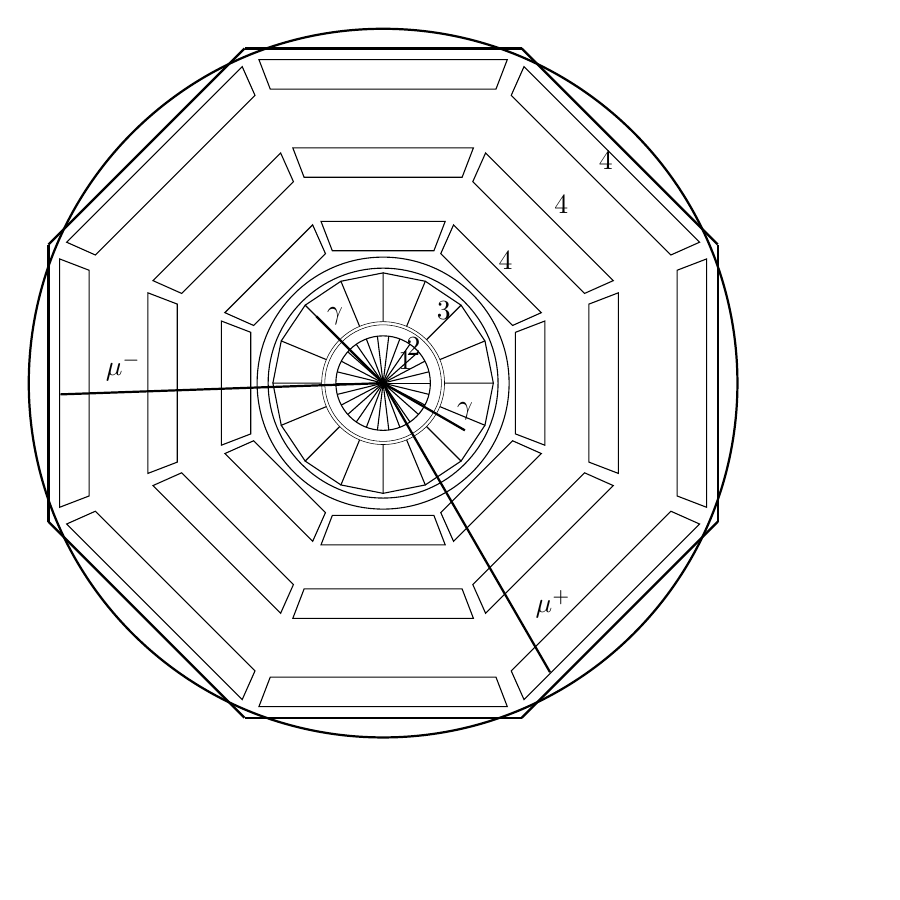
\begin{tikzpicture}[>=stealth,scale=2]
		\draw[white] (-1.1,-3.1) rectangle (3.1,0); % comment this line out, if you use the code.
		% Pic
		% Big circle
		\draw[black,thick] (0,0) circle (2.25);
		
		% small circle center
		\draw (0,0) circle (.3);
		\foreach \i in {0,13.85,27.7,41.55,55.4,69.25,83.1,96.95,110.8,124.65,138.5,152.35,166.2}{
			\draw ({0.3*cos(\i)},{0.3*sin(\i)}) -- ({-0.3*cos(\i)},{-0.3*sin(\i)});
		}
		\draw[very thin] (0,0) circle (.37);
		\draw[very thin] (0,0) circle (.39);
		
		\foreach \i in {0,22.5,45,67.5,90,112.5,135,157.5,180,202.5,225,247.5,270,292.5,315,337.5}{
			\draw ({.39*cos(\i)},{.39*sin(\i)}) -- ({.7*cos(\i)},{.7*sin(\i)}) -- ({.7*cos(\i+22.5)},{.7*sin(\i+22.5)});
		}
		\draw (0,0) circle (.73);
		\draw (0,0) circle (.8);
		\foreach \an in {0,45,90,135,180,225,270,315}{
			\draw ({.9*cos(\an-21)},{.9*sin(\an-21)}) -- ({.9*cos(\an+21)},{.9*sin(\an+21)}) -- ({1.1*cos(\an+21)},{1.1*sin(\an+21)}) -- ({1.1*cos(\an-21)},{1.1*sin(\an-21)}) -- cycle;
			\draw ({1.4*cos(\an-21)},{1.4*sin(\an-21)}) -- ({1.4*cos(\an+21)},{1.4*sin(\an+21)}) -- ({1.6*cos(\an+21)},{1.6*sin(\an+21)}) -- ({1.6*cos(\an-21)},{1.6*sin(\an-21)}) -- cycle;
			\draw ({2*cos(\an-21)},{2*sin(\an-21)}) -- ({2*cos(\an+21)},{2*sin(\an+21)}) -- ({2.2*cos(\an+21)},{2.2*sin(\an+21)}) -- ({2.2*cos(\an-21)},{2.2*sin(\an-21)}) -- cycle;
			\draw[thick] ({2.3*cos(\an-22.5)},{2.3*sin(\an-22.5)}) -- ({2.3*cos(\an+22.5)},{2.3*sin(\an+22.5)});
		}
		
		% gamma
		\draw[thick] (0,0) -- ({.6*cos(330)},{.6*sin(330)});
		\draw[thick] (0,0) -- ({.6*cos(135)},{.6*sin(135)});
		% mus
		\draw[thick] (0,0) -- ({2.05*cos(182)},{2.05*sin(182)});
		\draw[thick] (0,0) -- ({2.12*cos(300)},{2.12*sin(300)});
		% Beschriftungen
		\node[scale=1,right,very thick] at ({.6*cos(135)},{.6*sin(135)}) {$\gamma$};
		\node[scale=1,above,very thick] at ({.6*cos(330)},{.6*sin(330)}) {$\gamma$};
		\node[scale=1,above right,very thick] at ({1.8*cos(300)},{1.8*sin(300)}) {$\mu^{+}$};
		\node[scale=1,above,very thick] at ({1.65*cos(182)},{1.65*sin(182)}) {$\mu^{-}$};
  		\node[scale=1] at ({.2*cos(45)},{.2*sin(45)}) {1};
		\node[scale=1] at ({.3*cos(50)},{.3*sin(50)}) {2};
		\node[scale=1] at ({.6*cos(50)},{.6*sin(50)}) {3};
		\node[scale=1] at ({1.1*cos(45)},{1.1*sin(45)}) {4};
		\node[scale=1] at ({1.6*cos(45)},{1.6*sin(45)}) {4};
		\node[scale=1] at ({2*cos(45)},{2*sin(45)}) {4};
	\end{tikzpicture}
	
\end{document}
